\chapter{Application Development}

\section{Requirements (and Specifications)}


\section{Useful concepts definition}

More detailed explanations of the following concepts will be given later on, but it is helpful to shortly define them here so this work is more easily readable.

\subsection{Wallet} A password wallet is a digital form of securely keeping passwords and some meta information. In this work, a Wallet is stored as a Sqlite DataBase. A wallet can have as many tables as the user wants. For instance an user could have a table for storing social media passwords, another one for work-related passwords and a last one for credit cards and bank accounts passwords. Finally, Each table has a set of defined fields (Username, Domain, Password, Date, Description).

\subsection{SEcube} SEcube is a custom chip produced by the Blu5 group \cite{Blu5} that integrates a ARM CPU, and FPGA and a SmartCard. The chip is specifically designed for security purposes, allowing developers to implement encryption/decryption functions that are executed fast and are guaranteed to be reliable. The chip can be connected to a PC by USB, Ethernet etc...., so an application running on the PC can use the SEcube to encrypt/decrypt some date.

\subsection{SEcube SDK} The SEcube Open SDK is a set of open libraries designed to make the development of applications using SEcube more convenient. There are two types of Libraries: Host side (PC) and device side (SEcube) libraries. In general host side functions make requests to device side functions and wait for their response. Moreover, Libraries are divided in four and two hierarchical levels of abstraction, for host and device side respectively. Level0 and Level1 are the lowest levels and are present in both host and device. L0 provides the communication protocols while L1 provides basic security APIs.

\subsection{SEfile} 
SEfile is a Level 2 API that allows users to encrypt/decrypt data (files in the hard disk), so they can only be read when the SEcube chip is connected to the PC. When the SEcube is not connected, it is impossible to read the files as the information necessary to decrypt them is physically stored in the SEcube.

\subsection{Sqlite DB}


\section{Design}

The purpose of this section is to give the reader a clear overview of how the application works in general terms. 

A simplified design architecture is displayed in figure \ref{fig:BasicDesign}. It shows which Software Libraries are used by the application and when it uses them.


\begin{figure}[ht]
	\centering
	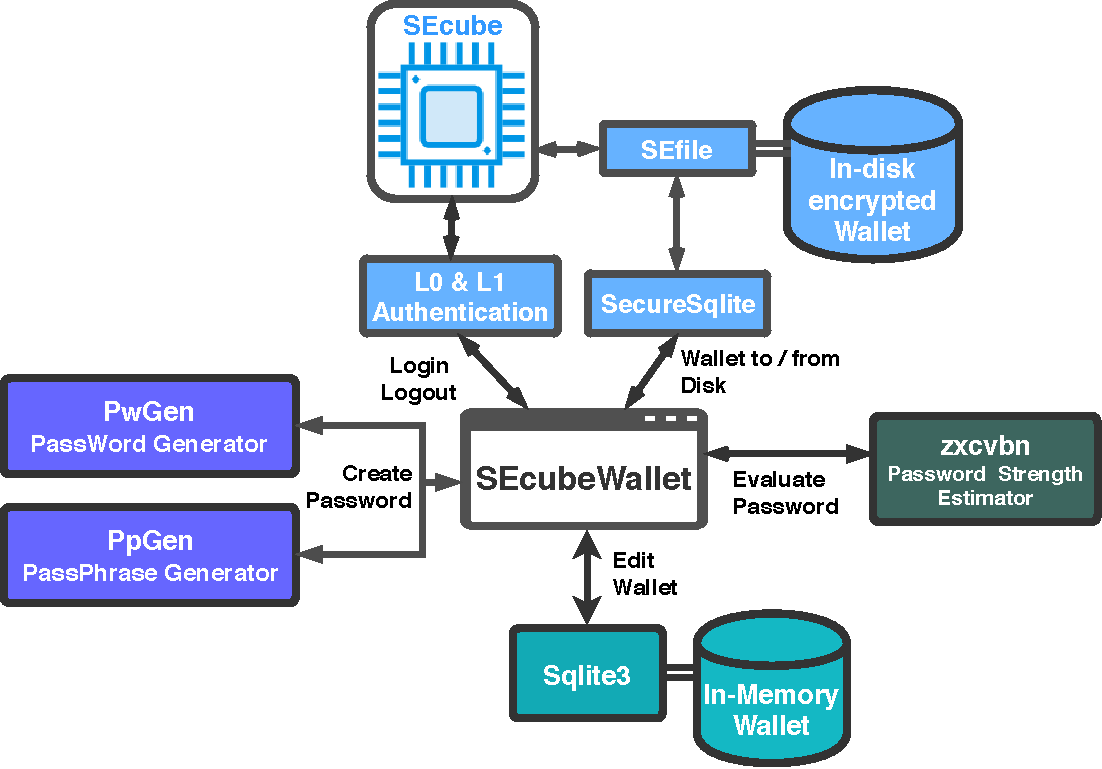
\includegraphics[width=\textwidth]{chapters/figures/development/BasicDesign.pdf}
	\caption{Basic Design: Used Libraries}
	\label{fig:BasicDesign}
\end{figure}

The following is a brief explanation of these Libraries and they usage. More details about each Library and why they were chosen are given in section \ref{sec:lib} and section \ref{sec:imp} deals with the actual implementation.

\subsection{L0 and L1 Authentication libraries}

When the user starts the application the first steps to perform are to open the communication with the device using Level0 functions from both host and device, and to authenticate the user by checking the login pin, using Level1 functions (again, from both sides). In the basic design diagram we can see how the SEcubeWallet uses the authentication functions and they in turn communicate with the SEcube chip.

\subsection{SecureSqlite3}
As explained before, Wallets are stored as Sqlite DataBases. Fortunately, the SEcube SDK already provides a Level2 API for creating and managing encrypted Sqlite DBs, called SecureSqlite3. This API exploits the SEfile API to wrap some of the functions of the original Sqlite3 library, avoiding OS calls.

SecureSqlite allows to create/edit/save/open databases that when written to the disk are encrypted and can only be read when the SEcube is connected. Additionally, as it is implemented using wrappers, the developer only needs to include the source files in the project and can manage SecureSqlite DB with the same functions used for regular Sqlite DB.

We can see in the diagram the SEcubeWallet application using SecureSqlite to read/write the encrypted wallet stored in disk.

\subsection{Sqlite3}
Because the use of SecureSqlite involves a call to the SEcube, a regular Sqlite3 DB is also used, but this DB is never saved to the disk. Sqlite3 allows for the creation of an In-Memory DB, i.e. a DB whose content is always in the memory space of the application an therefore secure by the operating system. 

The In-memory DB is used for editing. When the user want to save the wallet, i.e. write it to the disk, the contents of the In-Memory DB are dumped to the encrypted SecureSqlite DB. When the user opens a wallet from the disk, the reverse process occurs.

With the In-memory DB, unnecessary calls to the SEcube are avoided while maintaining the contents secured.

\subsection{Password Generator PwGen}
As the purpose of the application is to securely store passwords, said passwords should be as strong as possible. It does not make sense to protect a password that can be easily cracked by a hacker using brute force. That is why the application also includes a Password Generator.

PwGen is an open source library that generates passwords, that can either be easy to remember, or completely random. Random passwords are more secure, but as the are difficult to remember, their use only makes sense when the user stores them in a wallet manager. Among other aspects, length and characters used (Numbers, Upper cases) can be configured too.

When the user is adding a new entry to a wallet, they can chose to enter a password or to automatically generate one.

\subsection{Strength Estimator zxcvbn}
To give the users feedback on how good the password they are about to store is, the application uses the open source project zxcvbn to give an estimation of the passwords entropy, and how long it would take for a hacker to break it. zxcvbn bases its calculation in a number of factors, among them if the password is a common word, or a combination of them, a last name, a date, or letters close to each other in a keyboard (thus the name zxcvbn). With the estimator users are encouraged to create good passwords that are not necessarily completely random and difficult to remember, or annoying to type.

%\vspace{15pt} 
\vskip 25pt

To recap, these are the key aspects of the used libraries:

\begin{itemize}
\setlength\itemsep{0pt}
\item To start the connection with the SEcube, the Level0 library is used
\item To authenticate the user, by checking if the entered login pin is the same as the pin stored in the SEcube, the Level1 library is used.
\item An in-memory database is used for editing the wallet.
\item An encrypted in-disk data base is used for storing the wallet in disk.
\item The application includes a password generator with several options.
\item The application also includes a password strength estimator, so the user has an idea of how good their passwords are.

\end{itemize}

\section{Frameworks, Libraries and software tools} \label{sec:lib}

As explained in the previous section, the core of the design is the use of the SEcube chip to perform security operations in order to encrypt/decrypt some data stored in the host (PC). The requests to the chip are made from the Qt application developed in this work, which runs in the host. Said application exploits the existing C libraries SEfile and SecureSqlite to ease the communication with the SEcube. Additionally, the application also makes use of a random password generator PwGen and a strength estimator zxcvbn open libraries. 

In the following sections a review of the SEcube platform's hardware and software components is given. Then a brief explanation of the C++/Qt framework and why it was chosen. Finally the additional used libraries are presented.

\subsection{The SEcube framework}

"The SEcube™ (Secure Environment cube) Open Security Platform is an open source security oriented hardware and software platform, designed and constructed with ease of integration and service-orientation in mind. The hardware part of the platform was originally designed by Blu5 Group \cite{Blu5}, whereas the software libraries stem from a strong cooperation among international research institutions." \cite{GetStart}.

\vspace{5pt}

The main \textbf{hardware} products, explained in detail in the following sections, are:
\begin{itemize}
\setlength\itemsep{0pt}
\item The Chip, named SEcube Chip, or simply \textbf{SEcube}
\item The Development Board, named \textbf{SEcube DevKit}
\item The USB Stick, named \textbf{USEcube Stick}.
\end{itemize}

The SEcube chip is the main hardware component, and both the devkit and USB Stick are designed around it.The Development Board provides several communication protocols as well as debugging capabilities. For the final product the board would be of course too inconvenient to carry, and instead the USEcube Stick is preferred.

\subsection{The SEcube Chip}

"The SEcube™ (Secure Environment cube) is a powerful chip which
integrates three key security elements in a single package. A fast
floating-point Cortex-M4 \textbf{CPU}, a high-performance \textbf{FPGA} and an
EAL5+ certified Security Controller (\textbf{Smart Card}).
The result of this innovative combination gives an extremely
versatile secure environment in a single SoC, in which developers
can rapidly implement complex applications and appliances.
... The SEcube™ is the ultimate solution for high-end design,
delivering integration of a flexible, configurable and certified
secure element." \cite{SEcubeDS}

We can then see the SEcube chip as a powerful device offering the flexibility of an \textsc{ARM} CPU, the speed of an FPGA and the reliable security of a certified Smart Card, all bounded together and easily integrated in any project thanks to the available communication protocols, among them USB, UART, Ethernet and JTAG. 

The chip includes a true random number generator which relies in 240 noise seeds, all physical and therefore unpredictable. This allows the creation of true random noise. Additionally the user can choose what type of noise they want to generate, for instance white or Fourier noise.

%TODO
\todo{talk more about cpu, low power modes...}

In figure \ref{fig:SEcubeBD} a simplified SEcube architecture is shown.

\begin{figure}[ht]
	\centering
	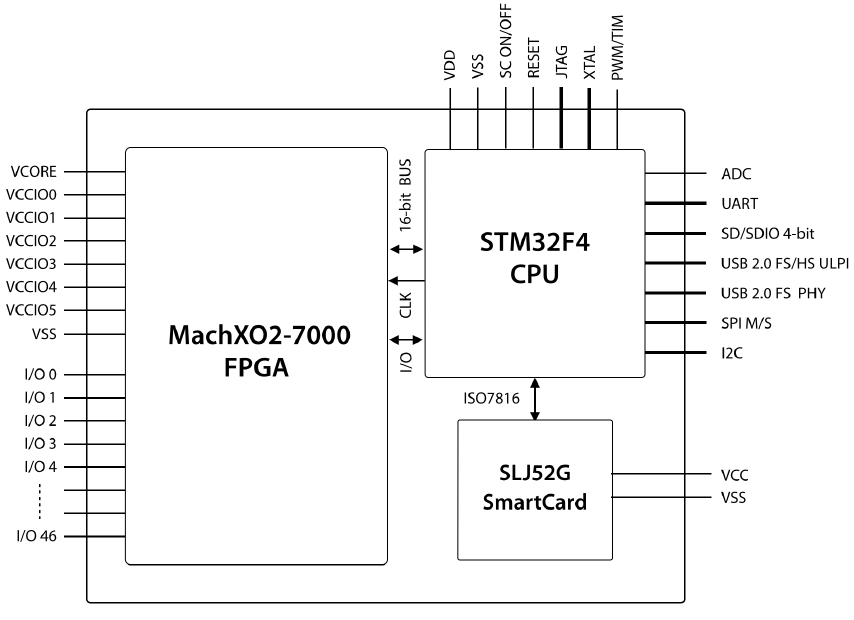
\includegraphics[width=\textwidth]{chapters/figures/development/SEcubeBlocks.png}
	\caption{SEcube Block Diagram}
	\label{fig:SEcubeBD}
\end{figure}


\subsection{Development board: The SEcube DevKit}

The development board integrates the SEcube chip with several peripherals that allow the user to easily communicate, program and debug. (Figure \ref{fig:devboard})

\begin{figure}[ht]
  \centering
  \subfloat[]{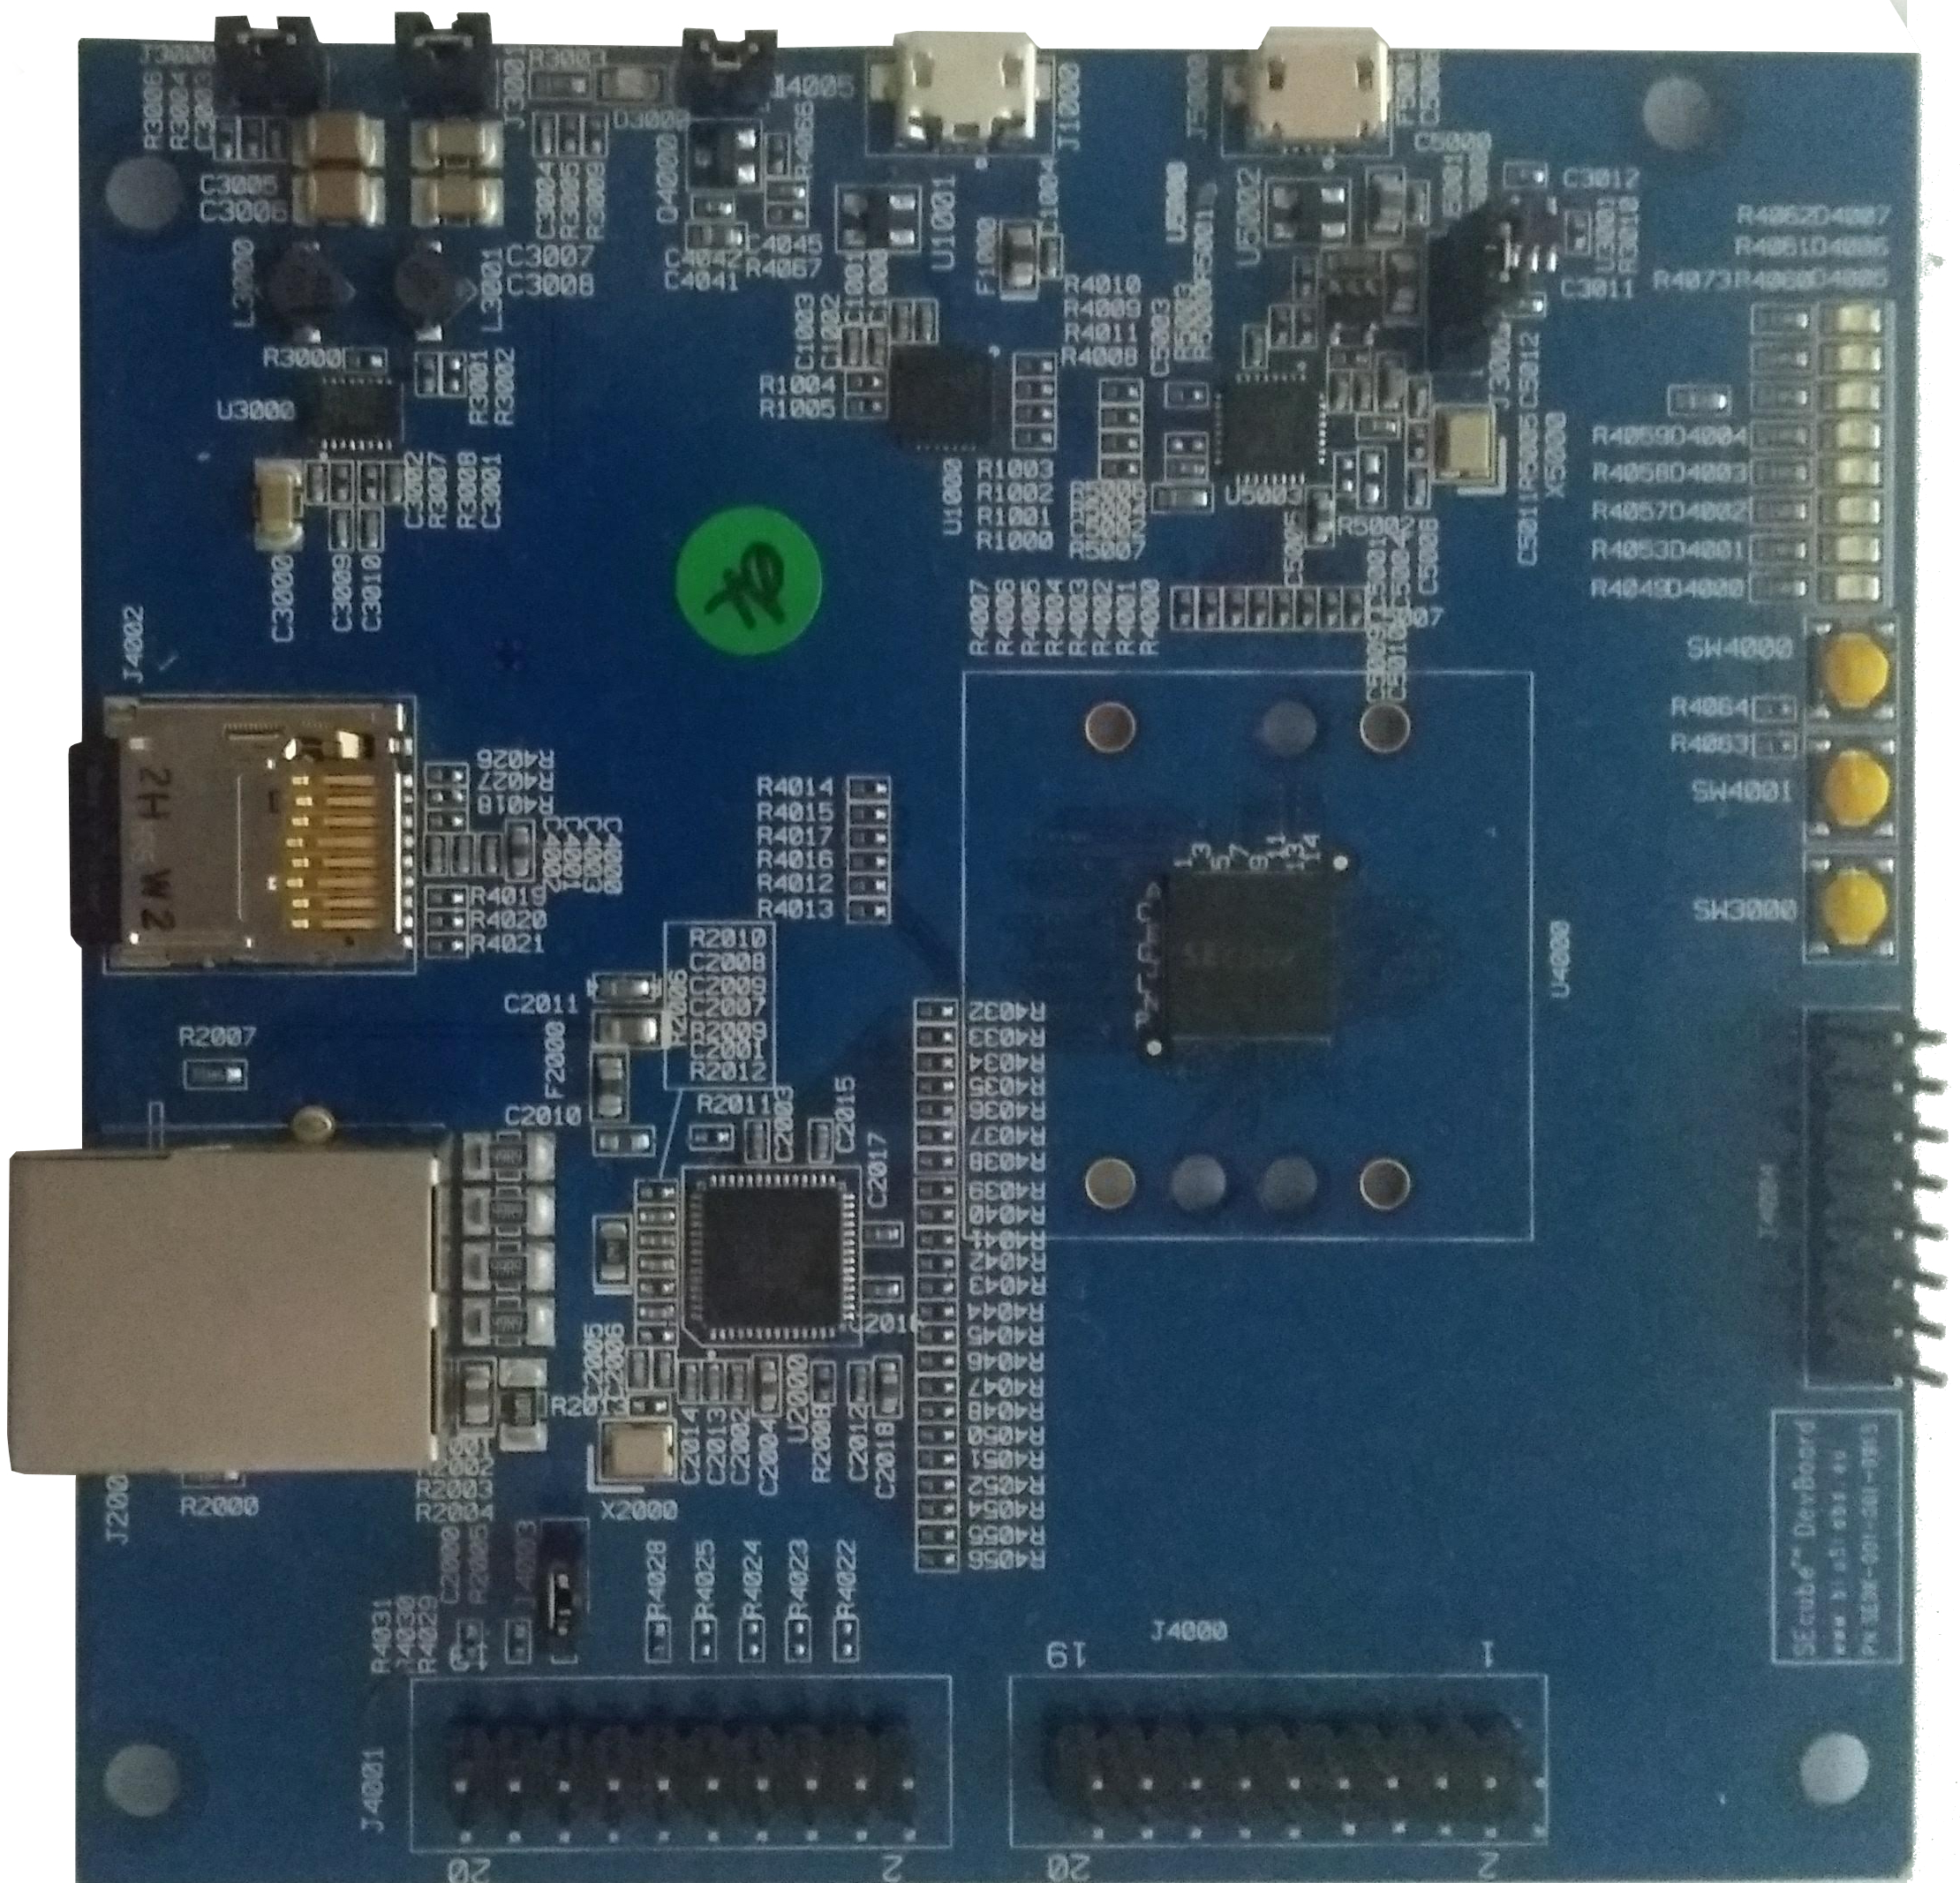
\includegraphics[width=0.485\textwidth]{chapters/figures/development/devboard.jpg}}
  \subfloat[]{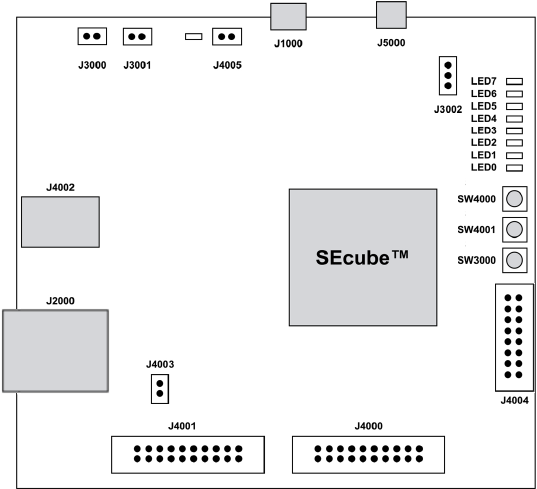
\includegraphics[width=0.515\textwidth]{chapters/figures/development/devboard_sch.png}}
  \caption{SEcube Devkit}
 \label{fig:devboard}
\end{figure}

The main peripherals in the SEcube devkit are:

\begin{itemize}
\setlength\itemsep{0pt}
\item \textbf{J1000: }\tabto{2.3cm} USB 2.0 to UART 
\item \textbf{J2000: }\tabto{2.3cm} Ethernet 10/100 socket 
\item \textbf{J4000: }\tabto{2.3cm} SEcube embedded FPGA and CPU GPIOs
\item \textbf{J4001: }\tabto{2.3cm} SEcube embedded CPU JTAG
\item \textbf{J4002: }\tabto{2.3cm} microSD card 
\item \textbf{J4004: }\tabto{2.3cm} SEcube embedded FPGA and CPU GPIOs
\item \textbf{J5000: }\tabto{2.3cm} USB 2.0 High Speed 
\item \textbf{LEDx:  }\tabto{2.3cm} Leds 
\item \textbf{SWx00y:}\tabto{2.3cm} Switches 
\end{itemize}

\subsection{Final product: USEcube Stick}

For the final product, its is desired that the user carries all the SEcube functionalities in a small and convenient package, so they can encrypt/decrypt the passwords in any PC by just connecting the USEcube Stick and running the SEcubeWallet application.

The USEcube Stick is compatible with any Operating System and the SEcube functionalities are easily exposed to applications and services without installing any driver.

The USEcube offers only the strictly required components: The SEcube chip, a USB 2.0 High-Speed interface and an SDcard socket. See Figure \ref{fig:USEcube} for more details.


Since the USEcube Stick storage capability is based on a external microSD card, the security of the system is improved, as this allows to have a separation of encrypted data from the encryptor/decryptor. Additionally, both the size and the speed can be tuned per the user requirement and can be changed at any time, just replacing the microSD, without buying a new USEcube Stick.
The microSD card socket is embedded in the USB connector allowing to save space making the USEcube Stick very compact and, at the same time dust
and water-resistant.
Since the USEcube Stick is not provided with the JTAG interface, to inject the firmware previously developed and tested on the SEcube DevKit, all the devices come with an embedded secure boot loader.


\begin{figure}[ht]
  \centering
  \subfloat[]{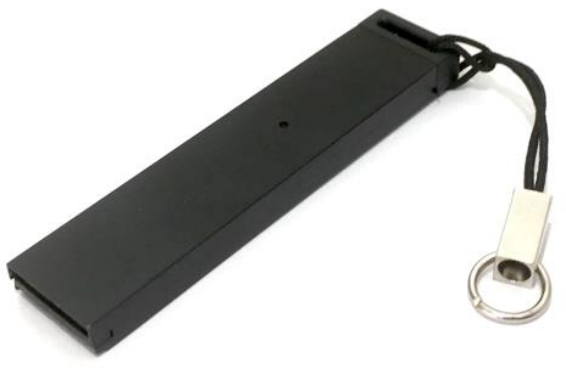
\includegraphics[width=0.485\textwidth]{chapters/figures/development/usb.png}}
  \subfloat[]{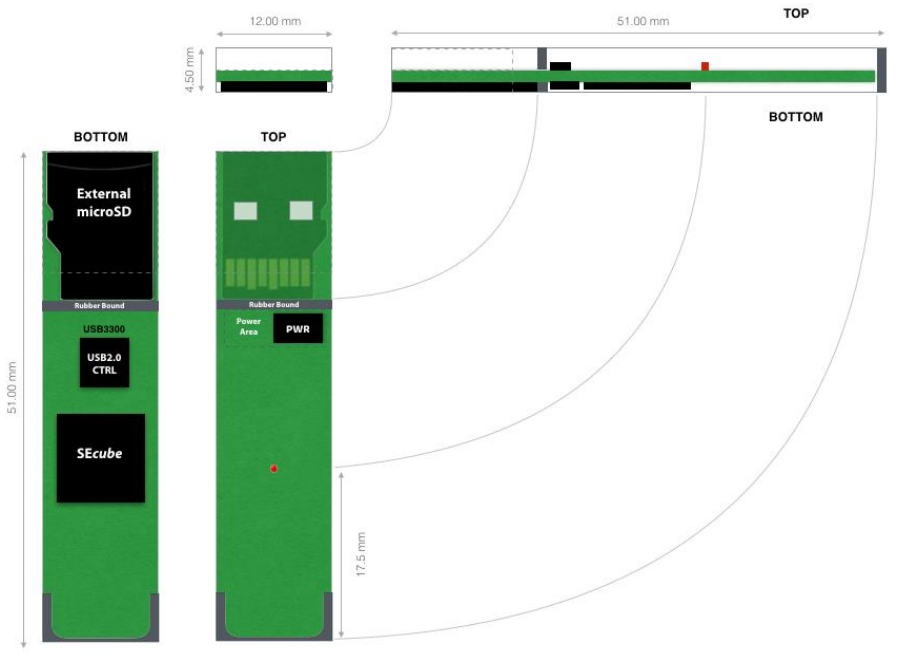
\includegraphics[width=0.515\textwidth]{chapters/figures/development/usb_sch.png}}
  \caption{USEcube Stick}
 \label{fig:USEcube}
\end{figure}


\subsection{L2 Security APIs}

"The software libraries and design environment allow developers who are not willing or able to produce the security APIs and protocols themselves to exploit the ready functions provided (currently as APIs and soon as services) within the SEcube platform and experience the platform as a high-security black box." \cite{L2UserMan}





"From the user/developer point of view, the APIs have been implemented targeting two
nested environments depending on where physically the code runs:
\begin{itemize}
\item \textbf{Device-Side}, including the libraries of basic functionalities that are executed on the embedded processor of the SEcube™-based hardware device.
\item \textbf{Host-Side}, containing libraries of functions executed on the host PC and interface functions for calling services and processes residing on the embedded processor of the SEcube™ device.
\end{itemize} 

From the architectural point of view, the Host-Side Libraries have been implemented targeting 4 hierarchical abstraction levels, and namely:
\begin{itemize}
\item \textbf{Level 0:} Communication Protocol and Provisioning APIs
\item \textbf{Level 1:} Basic Security APIs (Level1 Host-Side – L1)
\item \textbf{Level 2:} Intermediate Security APIs (Level2 – L2)
\item \textbf{Level 3:} Advanced Security APIs (Level3 – L3).
\end{itemize}

At each level, each component represents a "service" for the upper level and relies on "services" provided by the next lower level, only." \cite{L2UserMan}

"Level L2 relies on L1 services to provide the APIs for implementing more abstract secure functionalities. Typical examples include APIs for the protection of data both at rest and in-motion, or negotiating parameters (e.g., keys, algorithms) for establishing secure sessions, without being forced to understand in details all the low-level hardware and security mechanisms."\cite{L2UserMan}

L2 can be considered as the merge of two projects: \textbf{SEfile}, concerning data at rest, and \textbf{SElink}, concerning instead data at motion.

For our project we rely heavily on the development tools provided by the SEfile project, for the secure storage, usage and retrieve of data that requires a high degree of confidentiality, in our case, digital passwords.

\subsubsection{SEfile}

"SEfile targets any user that, by moving inside a secure environment, wants to perform basic operation on regular files. It must be pointed out that all encryption functionalities are demanded to the secure device in their entirety. In addition, SEfile does not expose to the host device details about what, or where it is reading/writing data: thus, the host OS, which might be untrusted, is totally unaware of what it is writing". \cite{L2UserMan}.

\subsubsection{SecureSqlite}

\subsection{Sqlite3}

\subsection{Graphical User Interface: the Qt framework}
The application's graphical user interface was developed using the \textbf{Qt framework}, version 5.8.0. 

"Qt is a cross-platform application development framework for desktop, embedded and mobile. Supported Platforms include Linux, OS X, Windows, VxWorks, QNX, Android, iOS, BlackBerry, Sailfish OS and others. Qt is not a programming language on its own. It is a framework written in C++. A preprocessor, the MOC (Meta-Object Compiler), is used to extend the C++ language with features like signals and slots. Before the compilation step, the MOC parses the source files written in Qt-extended C++ and generates standard compliant C++ sources from them. Thus the framework itself and applications/libraries using it can be compiled by any standard compliant C++ compiler like Clang, GCC, ICC, MinGW and MSVC".\cite{Qt}  


For writing, compiling and debugging source code, the IDE \textbf{Qt Creator}, version 4.2.1 was used.

"Qt Creator provides a cross-platform, complete integrated development environment (IDE) for application developers to create applications for multiple desktop, embedded, and mobile device platforms, such as Android and iOS. It is available for Linux, macOS and Windows operating systems".\cite{QtC}.

\vspace{5pt}
The reasons behind the use of Qt are as follows:

\begin{itemize}
\item Qt is a C++ library, and as such, allows for a seamless use of the C libraries SEfile and SecureSqlite, which are the backbone of this project.

\item Qt is cross-platform, meaning the developed application can be compiled to work on any of the major OSes. In particular, the development was carried out an tested on a Linux machine, but the application should work with no problems in Windows and MacOS. 

\item Because of good designed and ready-to-use display items such as tables, menus and dialogues, it is possible to focus in writing the functional portions of the application without worrying too much about the GUI. And as it is open source, any Qt item can be modified and extended when it does not meet the expectations out of the box. In this project several display elements were improved, as will be seen in section \ref{Implementation}.

\item Thanks to the multitude of functions dedicated to ease the use of C++ libraries and OS calls, one can be more productive, and the resulting code is more reliable. For instance, this project makes extensive use of such libraries, like QSqlDatabase, QString, QProcess, etc. Again, more details are given in section \ref{sec:imp}

\item Related works by research group \textsc{testgroup} from Politecnico di Torino using the SEcube framework, are written in Qt. Namely SecureSqliteBrowser and SEfile\_TXT, were used as base in the initial stages of development. This two projects can be found in the SEfileSDK available online \cite{SEcubeRes}.
%TODO
\todo{research group name  TESTGROUP?}

\item Qt is widely used, meaning it is possible to find tons of documentation, forums and additional libraries on the web. This also ensures the Qt framework will have continuous support from the developers and the community.

\end{itemize}



\subsection{PwGen: Random Password generator}

\subsection{zxcvbn: Password strength estimation}

\subsection{Device side development: Eclipse}

\section{Implementation} \label{sec:imp}


